\section{Structural changes during collective evolution}\label{sec:evolution}
Let $x_0$ be a state with $D(x_0)\ne\emptyset$ and $x_n=C^n(x_0)$, $D_n=D(x_n)$, $K_n=K(D_n)$. By \cref{lem:M-cited} $D_0\subseteq D_1\subseteq\cdots$, but the complexes $K_n$ are not nested: new occurrences pierce intervals and kill edges. The question is which structural features persist.

\subsection{Connectivity is governed by prime supports}
\begin{lemma}[component rule]\label{lem:comp}
For a finite $D\subset\Z_{\ge2}$ the components of $K(D)$ are the classes of the equivalence relation on $D$ generated by $u\approx v\iff\gcd(u,v)>1$. Equivalently $\beta_0(K(D))$ is the number of connected components of the bipartite graph between $D$ and the set of primes dividing elements of $D$ (with $d\sim p$ iff $p\mid d$).
\end{lemma}
The proof is in Appendix~\ref{app:proofs}; it uses only the interval criterion \cref{thm:A5T31-cited}: a coprime pair is never an edge because $1\in I(u,v)$, and a pair with $\gcd>1$ is joined by a path obtained by induction on $|I(u,v)|$. The lemma was also checked on $3000$ random sets (Appendix~\ref{app:finite}).
\begin{proposition}[\SIV{6}: hierarchy of structural persistence under evolution]\label{prop:P6}\status{new, proved; (d) uses cited census}
Along an orbit:
\begin{enumerate}[label=(\alph*),itemsep=1pt]
\item \emph{Vertices} persist: $D_n\subseteq D_{n+1}$.
\item \emph{Connectivity} persists: if $u,v\in D_n$ lie in one component of $K_n$ they lie in one component of $K_{n+1}$. Hence each component of $K_n$ is contained in a unique component of $K_{n+1}$, and $\beta_0$ changes only by merging old components and by adding components consisting of new vertices; a component never splits.
\item \emph{Edges} do not persist in general: a pair $\{u,v\}$ is an edge during exactly the interval $[\max(a(u),a(v)),p(u,v))$ of \cref{prop:P3}(b). In particular an edge that is lost is never regained.
\item \emph{Degrees $0$ and $1$ are not monotone.} For arbitrary inclusions of finite sets $D\subseteq D'=D\cup N$ of integers $\ge2$ (abstract transitions, not claimed to be occurrence inventories of rational states or steps of an orbit) there are exact witnesses for both directions of change in each of the two degrees: $\Delta\beta_0=-1$ for $D=\{3,10\}$, $N=\{18\}$ ($\beta_0:2\to1$) and $\Delta\beta_0=+1$ for $D=\{6,9\}$, $N=\{3,5\}$ ($1\to2$); $\Delta\beta_1=+1$ for $D=\{8,12\}$, $N=\{2\}$ ($\beta_1:0\to1$) and $\Delta\beta_1=-1$ for $D=\{5,14,33,60,90\}$, $N=\{6\}$ ($\beta_1:3\to2$). On realised orbits, the census of \Src{III}{thm:A5T7} over $2{,}576$ occurrence events has $\beta_1$ decreasing in $176$ and increasing in $388$, so degree $1$ is non-monotone along the examined orbits. Orbit-level non-monotonicity of $\beta_0$ is \emph{not} established by the abstract witnesses: for instance $D=\{3,10\}$ is not the occurrence set $D(x)$ of any state $x$, since $3,10\in D(x)$ force the denominator $b$ to divide both $2$ and $9$, hence $b=1$, and then $10\in D(x)$ forces $2\in D(x)$. For degree $2$ the census records changes in $246$ events and for degree $3$ in one event; no direction of change is claimed there, and monotonicity of $\beta_2,\beta_3$ is not decided by this paper.
\end{enumerate}
In particular the persistence is strictly graded: vertices $\supsetneq$ connectivity relation $\supsetneq$ edges, with homology of positive degree unconstrained beyond \Src{III}{thm:cause}.
\end{proposition}
\begin{proof}
(a) is \cref{lem:M-cited}. (b) By \cref{lem:comp} $u,v$ are in one component of $K_n$ iff they are joined by a chain $u=w_0,\dots,w_s=v$ in $D_n$ with $\gcd(w_{i-1},w_i)>1$. The same chain lies in $D_{n+1}\supseteq D_n$. Components of $K_{n+1}$ either contain an old component or consist of new vertices, so $\beta_0(K_{n+1})=\#\{\text{classes of }D_{n+1}\}$ counts merged old classes once and new classes. (c) is \cref{prop:P3}(b). (d) The four set-level witnesses are recomputed exactly (Appendix~\ref{app:finite}, witness W9, abstract set level); for instance $\{3,10\}$ has two components (they share no prime) and $18$ shares primes with both, giving $\beta_0=2\to1$, while $\{6,9\}\cup\{3,5\}$ adds the isolated vertex $5$, giving $1\to2$. The events of \cref{fig:types} are further instances for degree $0$. The census statements are quoted from \Src{III}{thm:A5T7}(b); they are finite-exact, are not recomputed here, and are used only as existence statements. Strictness of the grading is witnessed by the same events together with (c) (an edge between old vertices is lost while the connectivity relation is unchanged, \cref{fig:interval}).
\end{proof}
\begin{remark}
\cref{prop:P6}(b) is a statement about the relation $\sim_n$ on $D_n$; it does not say that $\beta_0$ is monotone. It says that all non-monotonicity of $\beta_0$ comes from the two sources named.
\end{remark}

\noindent\Cref{fig:orbit} shows dormant-to-active structure along an actual collective trajectory.

\begin{figure}[t]\centering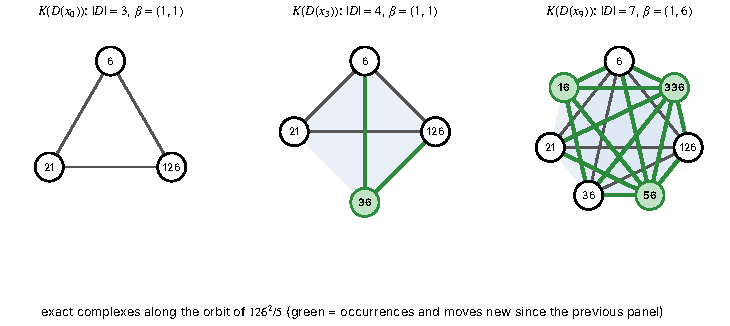
\includegraphics[width=\linewidth]{fig14_activation_orbit.pdf}
\caption{\textbf{Dormant-to-active structure along an actual collective trajectory.} Complexes $K(D(x_n))$ at $n=0,3,9$ of the orbit of $x_0=126^2/5$; green marks occurrences and moves that are new relative to the previous panel. The occurrence set grows, edges are born at arrival times. \emph{Exact complexes; vertex placement on a circle carries no meaning.}}\label{fig:orbit}\end{figure}
\begin{figure}[t]\centering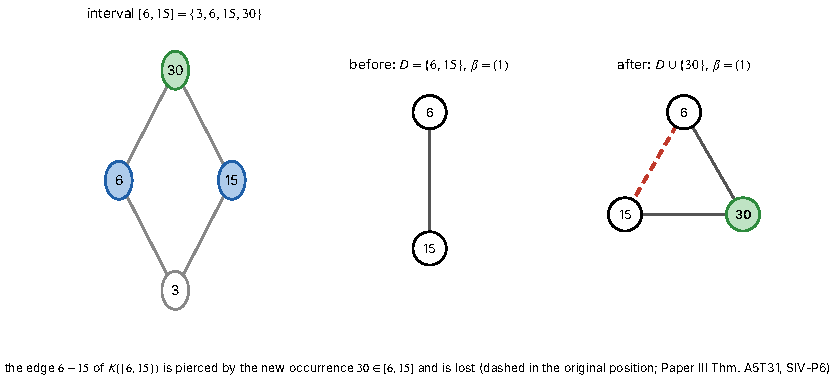
\includegraphics[width=\linewidth]{fig15_divisor_interval.pdf}
\caption{\textbf{Occurrence persistence with primitive-edge loss.} The divisor interval $I(6,15)=\{3,6,15,30\}$ and the complexes $K(\{6,15\})$ and $K(\{6,15,30\})$: the new occurrence $30$ pierces the interval and the edge $6$--$15$ is lost (dashed), replaced by $6$--$30$ and $15$--$30$ (\Src{III}{thm:A5T31}). \emph{Exact.}}\label{fig:interval}\end{figure}
\begin{figure}[t]\centering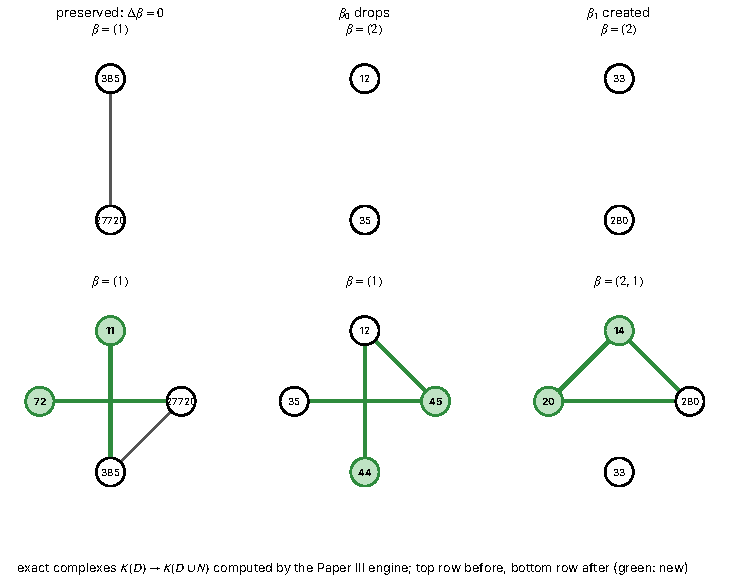
\includegraphics[width=\linewidth]{fig16_event_types.pdf}
\caption{\textbf{Topological creation, preservation and destruction.} Three exact events $K(D)\to K(D\cup N)$: unchanged Betti numbers, loss of a component, creation of a first homology class. \emph{Exact complexes computed by the engine of Paper~III; $\beta$ over $\mathbb F_2$.}}\label{fig:types}\end{figure}
